\documentclass[usenames,dvipsnames]{beamer}

\usetheme[
	progressbar=frametitle,
	titleformat section=smallcaps,
	subsectionpage=progressbar
]{metropolis}

\providecommand{\version}{local-dev}


% cSpell:disable
% chktex-file 15

% CLI arguments

\usepackage{ifthen}
\ifthenelse%
	{\equal{\generatenotes}{hide}}
	{\newcommand{\notesOption}{hide notes}}
	{
		\ifthenelse%
			{\equal{\generatenotes}{second}}
			{\newcommand{\notesOption}{show notes on second screen}}
			{\newcommand{\notesOption}{show only notes}}
	}%

% packages

\usepackage[
	orientation=landscape,
	size=custom,
	width=24,
	height=14,
	scale=0.6
]{beamerposter}

\usepackage{pgfpages}
\usepackage{booktabs}
\usepackage{bm}
\usepackage{mathtools}
\usepackage{listings}
\usepackage{fancybox}
\usepackage{bm}
\usepackage{multicol}
\usepackage{xpatch}
\usepackage{hyperref}
\usepackage{hyperxmp}
\usepackage{multirow}
\usepackage{xparse}
\usepackage{hyphenat}
\usepackage{xfrac}
\usepackage{caption}
\usepackage{enumitem}
\setitemize{label=	\usebeamerfont*{itemize item}
					\usebeamercolor[fg]{itemize item}
					\usebeamertemplate{itemize item}}

\usepackage{siunitx}
\sisetup{range-phrase=--}

\usepackage{natbib}
\bibliographystyle{natbib}

\usepackage{background}
\backgroundsetup{
	placement=center,
	scale=3,
	contents={\begin{minipage}{1.0\textwidth}\centering\wm\end{minipage}},
	opacity=0.02,
	color=gray,
	angle=0
}
\setbeamertemplate{background}{\BgMaterial}


% settings

\graphicspath{{./graphics/}}

\makeatletter
\defbeameroption{show only notes}[]%
{
	\beamer@notestrue%
	\beamer@notesnormalsfalse%
}
\makeatother

\setbeameroption{\notesOption}

\setsansfont{CMU Serif}
\setmonofont{CMU Typewriter Text}

\makeatletter
\let\@@magyar@captionfix\relax % chktex 21
\makeatother

\logo{
	
\includegraphics[
		width=2cm,
		keepaspectratio
	]{logo}\hspace{\dimexpr\paperwidth-2cm-10pt}\vspace{-30pt}
}

\titlegraphic{%
	\begin{picture}(0,0)
		\put(620,-180){\makebox(0,0)[rt]{
\includegraphics[width=5cm]{logo}}}
	\end{picture}
}

\makeatletter
	\def\beamer@framenotesbegin{% at beginning of slide
		\usebeamercolor[fg]{normal text}
			\gdef\beamer@noteitems{}%
			\gdef\beamer@notes{}%
	}
\makeatother

\definecolor{RoyalBlue}{RGB}{11,32,76}
\definecolor{DustyBlue}{RGB}{81,150,195}

\hypersetup{
	colorlinks=true,
	linkcolor=RoyalBlue,
	urlcolor=RoyalBlue,
	citecolor=DustyBlue,
	pdfpagemode=FullScreen,
	pdfdisplaydoctitle=true,
	pdfmenubar=false,
	pdfpagelayout=SinglePage
}

\captionsetup[figure]{labelformat=empty}

\makeatletter
	\setlength{\metropolis@progressinheadfoot@linewidth}{2pt}
\makeatother

\setbeamercolor{background canvas}{bg=white}
\setbeamercolor{normal text}{fg=RoyalBlue}
\setbeamercolor{alerted text}{fg=DustyBlue}
\setbeamercolor{example text}{fg=RoyalBlue}
{
	\usebeamercolor[fg]{alerted text}
	\usebeamercolor[fg]{example text}
	\usebeamercolor[fg]{normal text}
}

% definitions

\xpatchbibmacro{name:andothers}{%
	\bibstring{andothers}%
}{%
	\bibstring[\emph]{andothers}%
}{}{}

\makeatletter
	\newcommand{\manuallabel}[2]{\def\@currentlabel{#2}\label{#1}} % chktex 21
\makeatother

\newenvironment<>{fixblock}[1]{%
	\begin{block}{#1}
		\vspace{0pt}
		#2
}{
	\end{block}
}

\newenvironment{fixnote}{\startfixnote}{}
\def\startfixnote#1\end{\note{#1}\end} % chktex 9 chktex 14


\title{Dissertation Defense}

\subtitle{
	Secure and Efficient Query Processing in Outsourced Databases \\
	{\small Range Queries~\cite{ore-benchmark-17, epsolute}, Point Queries~\cite{epsolute}, \knn{} Queries}
}

\date{Built from \href{https://git.dbogatov.org/bu/defense/presentation/commit/\version}{\emph{\version}} on \today}

\author{Dmytro Bogatov \\ \email{dmytro@bu.edu}}

\institute{Boston University \\ Graduate School of Arts and Sciences \\ Department of Computer Science}

\def\wm{
\includegraphics[keepaspectratio, width=0.1\textwidth]{coat-of-arms-1}}


\begin{document}

	\maketitle

	
\setbeamercovered{transparent}
\newlength{\listLabelLength}

\section{Background}

	\begin{frame}{Motivation and overview}

		\begin{itemize}
			\item<1-> With vast amounts of data, organizations choose to use cloud solutions
			\item<1-> These solutions need to be both efficient and secure
			\item<2-> Recent attacks on access pattern (AP)~\cite{multidimensional-range-queries, inference-attack-islam-14, leakage-abuse-attacks-cash-15, inference-attacks-naveed-15, generic-attacks-kellaris, attacks-tao-of-inference, grubbs-attacks, access-pattern-disclosure, atacks-improved-reconstruction} and communication volume (CV)~\cite{generic-attacks-kellaris, state-of-uniform, atacks-improved-reconstruction, pump-volume-attacks, volume-range-attacks}
			\item<3->
				Existing solutions may be insufficient:
				\begin{itemize}
					\item<1,2,3,6-> \normalsize
						protection against snapshot adversary does not account for AP and CV \\
						\small{CryptDB~\cite{crypt-db}, Arx~\cite{arx}, Seabed~\cite{seabed} and SisoSPIR~\cite{sisospir}}

					\item<1,2,4,6-> \normalsize
						enclaves like SGX are still uncommon and limited in memory \\
						\small{Cipherbase~\cite{cipherbase}, HardIDX~\cite{hardidx}, StealthDB~\cite{stealth-db}, EnclaveDB~\cite{enclave-db}, ObliDB~\cite{oblidb}, Opaque~\cite{opaque} and Oblix~\cite{oblix}}

					\item<1,2,5,6-> \normalsize
						other solutions protect either from one of AP or CV, or use linear scan and full padding \\
						\small{\crypte~\cite{crypte}, Shrinkwrap~\cite{shrinkwrap}, SEAL~\cite{seal} and PINED-RQ~\cite{pined-rq}}
				\end{itemize}
			\item<6-> \epsolute{}: most secure and practical range- and point-query engine in the outsourced database model, that protects both AP and CV using Differential Privacy, while not relying on TEE, linear scan or full padding
		\end{itemize}

	\end{frame}

	\begin{frame}{Cryptographic primitives}

		\begin{columns}[T,onlytextwidth]
			\column{0.475\textwidth}

				\onslide<1->{

					\begin{block}{Symmetric Encryption Scheme}
						\vspace*{1ex}

						\settowidth{\listLabelLength}{\textbf{Key generation}}
						\begin{description}[
							font=\bfseries,
							leftmargin=\dimexpr\listLabelLength+1em\relax,
							labelindent=0pt,
							labelwidth=\listLabelLength%
							]
							\item[Key generation] $k \sample \algo{E.KeyGen}{}$
							\item[Encrypt] $c \sample \algo{E.Enc}{x, k}$
							\item[Decrypt] $x \gets \algo{E.Dec}{c, k}$
						\end{description}

					\end{block}
				}

			\column{0.475\textwidth}

				\onslide<2->{

					\begin{block}{Order-revealing encryption scheme}
						\vspace*{1ex}

						\settowidth{\listLabelLength}{\textbf{Key generation}}
						\begin{description}[
							font=\bfseries,
							leftmargin=\dimexpr\listLabelLength+1em\relax,
							labelindent=0pt,
							labelwidth=\listLabelLength%
						]
							\item[Key generation] $k \sample \algo{ORE.KeyGen}{}$
							\item[Encrypt] $c \sample \algo{ORE.Enc}{x, k}$
							\item[Decrypt] $x \gets \algo{ORE.Dec}{c, k}$
							\item[Compare] $c_1\ \texttt{op}\ c_2 \equiv x_1\ \texttt{op}\ x_2$ \\ $\texttt{op} \in \{ <, \le, =, \ge, > \}$
						\end{description}

					\end{block}
			}

		\end{columns}

		\vspace*{3ex}

		\begin{columns}[T,onlytextwidth]
			\column{0.475\textwidth}
				\onslide<1->{

						For example, AES~\cite{aes-nist} in CBC mode + IV~\cite{modes-of-operation-nist}.
				}

			\column{0.475\textwidth}
				\onslide<2->{

						For example, BCLO~\cite{bclo-ope}, CLWW~\cite{clww-ore}, Lewi-Wu~\cite{lewi-wu-ore}, CLOZ~\cite{cloz-ore} and FH-OPE~\cite{fh-ope}.
				}

		\end{columns}

		\note{
			The note.

		}

	\end{frame}

	\begin{frame}{Access pattern and ORAM}

		\justifying%

		\textbf{Access pattern} is a sequence of memory accesses \oramProgram{}, where each access consists of the memory \emph{location} $o$, read \oramRead{} or write \oramWrite{} \emph{operation} and the \emph{data} $d$ to be written.

		Oblivious RAM (ORAM) is a mechanism that hides the accesses pattern.
		More formally, \oram{} is a protocol between the client \client{} (who accesses) and the server \server{} (who stores), with a guarantee that the view of the server is indistinguishable for any two sequences of the same lengths.

		\begin{columns}[T]
			\column{0.475\textwidth}

				\[
					\begin{split}
						\abs{\oramProgram_1}					& = \abs{\oramProgram_2}							\\
						\textsc{View}_\server (\oramProgram_1)	& \cindist \textsc{View}_\server (\oramProgram_2)
					\end{split}
				\]

			\column{0.475\textwidth}

				\procedure[linenumbering]{\oram{} protocol}{
					\textbf{Client \client}											\>														\> \textbf{Server \server}	\\
					%
					\oramProgram{} = \left. (\oramRead, i, \bot) \right|_{i = 1}^5	\> 														\>							\\
					%
					\text{(client state)}											\> \sendmessageboth*[6em]{\algo{ORAM}{\oramProgram}}	\> \text{(server state)}	\\
					%
					\{ d_1, d_2, d_3, d_4, d_5 \}									\>														\>
				}

		\end{columns}

		\vspace*{1ex}

		For example: Square Root ORAM~\cite{oram-theory}, Hierarchical ORAM~\cite{oram-original}, Binary-Tree ORAM~\cite{binary-tree-oram}, Interleave Buffer Shuffle Square Root ORAM~\cite{shortest-path-oram}, TP-ORAM~\cite{tp-oram}, \textbf{Path-ORAM}~\cite{path-oram} and TaORAM~\cite{taostore}.
		\alert{ORAM incurs at least logarithmic overhead in the number of stored records.~\cite{oram-original}}

	\end{frame}

	\begin{frame}{Privacy}

		\begin{block}{$k$-anonymity~\cite{k-anonymity}}
			\justify%

			Every tuple in the released table must be indistinguishably related to no fewer than $k$ respondents (i.e., similar to at lest $k - 1$ other tuples).

			\begin{itemize}
				\item only with respect to quasi-identifiers
				\item attacks using background knowledge and lack of diversity
				\item a property of a table, not a mechanism (other works with anonymization techniques exist) % l-diversity page 3 bottom
			\end{itemize}
			% https://spdp.di.unimi.it/papers/k-Anonymity.pdf1

		\end{block}

		\pause%

		\begin{block}{$\ell$-diversity~\cite{l-diversity}}
			\justify%

			A block is $\ell$-diverse if it contains at least $\ell$ ``well-represented'' values for the sensitive attribute $S$.
			A table is $\ell$-diverse if every block is $\ell$-diverse.

			Can choose definition of ``well-represented''.
			For example, in \emph{entropy $\ell$-diversity}, every block has at least $\ell$ distinct values for the sensitive attribute.
			In \emph{recursive $\ell$-diversity}, most common value does not appear too often, less common --- not too infrequently.

			% https://personal.utdallas.edu/~muratk/courses/privacy08f_files/ldiversity.pdf

		\end{block}

		% security hides all data completely at a cost, privacy protects information of an individual from inference and de-anonymization

	\end{frame}

	\begin{frame}{Privacy}

		\begin{block}{$t$-closeness~\cite{t-closeness}}
			\justify%

			A block exhibits $t$-closeness if the distance between the distributions of a sensitive attribute in this block and in the whole table is no more than a threshold $t$.
			A table exhibits $t$-closeness if every block does.
			The metric used is the Earth Mover's Distance~\cite{emd}.

			% https://citeseerx.ist.psu.edu/viewdoc/download?doi=10.1.1.157.824&rep=rep1&type=pdf

		\end{block}

		\pause%

		\begin{block}{Differential Privacy, adapted from~\cite{our-data-ourselves, differential-privacy-original}}
			\justify%

			A randomized algorithm \algo{A} is $(\epsilon, \delta)$-differentially private if for all $\database_1 \sim \database_2 \in \searchKeyDomain^\dataSize$, and for all subsets $\mathcal{O}$ of the output space of \algo{A},
			\[
				\probability{ \algo{A}{ \database_1 } \in \mathcal{O} } \leq \exp(\epsilon) \cdot \probability{ \algo{A}{ \database_2 } \in \mathcal{O} } + \delta \; .
			\]

			\begin{itemize}
				\item Laplace Perturbation Algorithm (LPA)~\cite[Theorem 1]{differential-privacy-original}
				\item Differentially Private Sanitizer
				\item Composition Theorem (disjoint and non-disjoint sets)
			\end{itemize}

		\end{block}

	\end{frame}

	\begin{frame}{Encalves, SGX and ZeroTrace}

		\begin{block}{Software Guard Extensions (SGX)~\cite{sgx-1, sgx-2, sgx-3, sgx-manual, sgx-explained}}
			\justify%

			\vspace*{1ex}

			\begin{columns}[T,onlytextwidth]
				\column{0.6\textwidth}

					Features:
					\begin{itemize}
						\item Set of new x86 instructions
						\item Virtual isolation within ``enclaves''
						\item The entire non-enclave stack is untrusted
						\item Can swap/re-encrypt pages from RAM
						\item Application declares enclave and non-enclave parts
						\item Enclave should manipulate sensitive data, e.g., keys
					\end{itemize}

				\column{0.4\textwidth}

					Issues:
					\begin{itemize}
						\item Small $\approx \SI{96}{\mega\byte}$ of ``trusted'' memory
						\item Enclave code is significantly slower
						\item No direct I/O or syscalls
						\item \alert{Leaks access pattern}
					\end{itemize}

			\end{columns}

		\end{block}

		\vspace*{1ex}

		\begin{block}{ZeroTrace~\cite{zerotrace}}
			\justify%

			PathORAM~\cite{path-oram} or CircuitORAM~\cite{circuit-oram} in SGX, given that the enclave code leaks access pattern. Uses oblivious operations.

		\end{block}

	\end{frame}



	\section{Model}

	\begin{frame}{Snapshot adversary / Data-at-rest}

		\begin{columns}[T,onlytextwidth]
			\column{0.5\textwidth}

				\begin{block}{Adversary steals the hard drive}

					\begin{itemize}
						\item<1-> Cannot query fully encrypted blob \\ \small{cannot outsource key}
						\item<1-> Download-decrypt-query is inefficient
						\item<1-> Relaxing from absolute (semantic) security
						\item<2-> Searchable symmetric encryption (SSE)~\cite{sse-improved}
						\item<3-> Fully-homomorphic encryption (FHE)~\cite{fhe}
						\item<4-> Functional Encryption~\cite{functional-encryption}
						\item<5-> Property-preserving encryption (PPE)~\cite{ope-original, ore-original}
					\end{itemize}

				\end{block}

			\column{0.5\textwidth}

				\onslide<6,7>{

					\begin{block}{Attacks}

						\begin{itemize}
							\item<1-5,6-> Usually require auxillary knowledge \\ \small{e.g., distribution} % chktex 8
							\item<1-5,6-> Not necessarily ``full'' reconstruction % chktex 8
							\item<1-5,7-> Inference Attacks on Property-Preserving Encrypted Databases~\cite{inference-attacks-naveed-15} % chktex 8
							\item<1-5,7-> The Tao of Inference in Privacy-Protected Databases~\cite{attacks-tao-of-inference} % chktex 8
							\item<1-5,7-> Why Your Encrypted Database Is Not Secure~\cite{grubbs-attacks} % chktex 8
							\item<1-5,7-> Data Recovery on Encrypted Databases With k-Nearest Neighbor Query Leakage~\cite{knn-attacks} % chktex 8
						\end{itemize}

					\end{block}

				}

		\end{columns}

	\end{frame}

	\begin{frame}{Persistent adversary / AP and CV leakage}

		\begin{columns}[T,onlytextwidth]
			\column{0.5\textwidth}

			\onslide<1->{
				\begin{block}{Access Pattern}

					\begin{itemize}
						\item Which query ``touches'' which records
						\item Applicable to all types of queries
						\item Usually mitigated with ORAM
						\item Attacks~\cite{multidimensional-range-queries, inference-attack-islam-14, leakage-abuse-attacks-cash-15, inference-attacks-naveed-15, generic-attacks-kellaris, attacks-tao-of-inference, grubbs-attacks, access-pattern-disclosure, attacks-improved-reconstruction}
					\end{itemize}

				\end{block}
			}

			\column{0.5\textwidth}

				\onslide<2->{

					\begin{block}{Communication volume}

						\begin{itemize}
							\item The size of the answer (in bytes or records)
							\item More often applicable to range queries
							\item Usually mitigated with padding / noise
							\item Attacks~\cite{generic-attacks-kellaris, state-of-uniform, attacks-improved-reconstruction, pump-volume-attacks, volume-range-attacks}
						\end{itemize}

					\end{block}

				}

		\end{columns}

		\vspace*{2ex}

		\onslide<3->{
			Can we put forth a definition that would imply protection against all these attacks?
		}

	\end{frame}

	\begin{frame}{Differentially Private Outsourced Database System}

		\begin{definition}[\alert{Computationally Differentially Private Outsourced Database System (CDP-ODB)}]
			\justify%

			We say that an outsourced database system \protocol{} is $(\epsilon, \delta)$-computationally differentially private (a.k.a.~CDP-ODB) if for every polynomial time distinguishing adversary \adversary{}, for every neighboring databases $\database \sim \database^\prime$, and for every query sequence $\fromNtoM{\query}{1}{m} \in \querySet^m$ where $m = \mathsf{poly}(\lambda)$,

			\begin{multline*}
				\probability{\adversary \left( 1^\lambda, \view{\protocol, \server}{\database, \fromNtoM{\query}{1}{m}} \right) = 1 } \leq \\
				\exp{\epsilon} \cdot \probability{\adversary \left( 1^\lambda, \view{\protocol ,\server}{\database^\prime, \fromNtoM{\query}{1}{m}} \right) = 1} + \delta + \negl \; ,
			\end{multline*}
			the probability is over the randomness of the distinguishing adversary \adversary{} and the protocol \protocol{}.
		\end{definition}

		\pause%

		Note:
		\begin{itemize}
			\item Entire view of the adversary is DP-protected
			\item Implies protection against communication volume and access pattern leakages
			\item Query sequence $\fromNtoM{\query}{1}{m} \in \querySet^m$ is fixed
			\item $\negl$ accounts for the computational (as opposed to theoretical) DP definition
		\end{itemize}

	\end{frame}

	% cSpell:ignore ORAMs

\section{Work in the Area}

	\subsection{Property-Preserving Encryption}

		\begin{frame}{Survey of OPE/ORE schemes~\cite{ore-benchmark-17}}

			\begin{columns}[T,onlytextwidth]
				\column{0.5\textwidth}

					\begin{block}{The problem}

						\begin{itemize}
							\item Many different solutions
							\item Performance / security tradeoff
							\item Heterogeneous security definitions and leakage profiles
							\item \textbf{Performance of the schemes not well-understood}
							\begin{itemize}
								\item Some were not even implemented
								\item Prototype implementation at best
								\item Not benchmarked against one another
								\item Use different primitive implementations
							\end{itemize}
						\end{itemize}

					\end{block}

				\column{0.5\textwidth}

					\onslide<2->{
						\begin{block}{Our solution}

							\begin{itemize}
								\item Analyzed security and leakages of the constructions under a common framework
								\item Analyzed theoretically performance of the constructions
								\item \textbf{Implemented and run experiments}
								\begin{itemize}
									\item Implemented 5 OPE / ORE schemes and 5 range query protocols
									\item Used same language, framework and primitive implementations
									\item Benchmarked primitives execution times
									\item Counted primitives and I/O usage
								\end{itemize}
							\end{itemize}

						\end{block}
					}

			\end{columns}

		\end{frame}

		\begin{frame}{Survey of OPE/ORE schemes~\cite{ore-benchmark-17}}

			\begin{columns}[T,onlytextwidth]
				\column{0.4\textwidth}

					\begin{block}{OPE/ORE schemes + leakage}

						\begin{itemize}
							\item \normalsize BCLO~\cite{crypt-db-ope} \\ \small{$\approx$ top half of the bits}
							\item \normalsize CLWW~\cite{practical-ore} \\ \small{most-significant differing bit}
							\item \normalsize Lewi-Wu~\cite{lewi-ore} \\ \small{most-significant differing block}
							\item \normalsize CLOZ~\cite{adam-ore-v2} \\ \small{equality pattern of most-significant differing bit}
							\item \normalsize FH-OPE~\cite{fh-ope} \\ \small{insertion order}
						\end{itemize}

					\end{block}

				\column{0.6\textwidth}

					\begin{block}{Range query protocols + leakage (on top of result size)}

						\begin{itemize}
							\item \normalsize {\BPlus} tree with ORE \\ \small{same as underlying ORE}
							\item \normalsize Kerschbaum~\cite{florian-protocol} \\ \small{total order}
							\item \normalsize POPE~\cite{pope} \\ \small{partial order}
							\item \normalsize Logarithmic-BRC~\cite{practical-range-search} \\ \small{same as underlying SSE}
							\item \normalsize ORAM with {\BPlus} tree \\ \small{fully hiding}
						\end{itemize}

					\end{block}

			\end{columns}

		\end{frame}

		\begin{frame}{CryptDB~\cite{crypt-db}}

			\begin{columns}[T,onlytextwidth]
				\column{0.6\textwidth}

					\begin{block}{CryptDB design and contributions}

						\begin{itemize}
							\item Regular SQL API for applications
							\item Proxy between app and server rewrites queries
							\item Encryption depending on operations
							\begin{small}
								\begin{itemize}
									\item \algo{DET} for equality
									\item \algo{OPE} for comparison
									\item \algo{HE} for aggregates
									\item \algo{RND} if not used
								\end{itemize}
							\end{small}
							\item Records encrypted in onion layers
							\item Column key derives from user password
						\end{itemize}

					\end{block}

				\column{0.4\textwidth}

					\begin{block}{Issues}

						\begin{itemize}
							\item Once onion level is removed, security degradation is permanent
							\item Leakage
							\begin{itemize}
								\item Order and histogram
								\item Access pattern
								\item Communication volume
							\end{itemize}
						\end{itemize}

					\end{block}

			\end{columns}

		\end{frame}

		\begin{frame}{Arx~\cite{arx}, PPQED~\cite{ppqed} and SisoSPIR~\cite{sisospir}}

			\begin{columns}[T,onlytextwidth]
				\column{0.5\textwidth}

					\begin{block}{Arx~\cite{arx}}

						\begin{itemize}
							\item A proxy between app and MongoDB
							\item Uses only semantically secure encryption
							\item Innovative range index with garbled circuits \\
							\begin{small} has to ``rebuild'' circuits \end{small}
							\item Equality index inspired by SSE
							\item Almost no leakage for snapshot adversary
							\item Requires schema and queries in advance
							\item \textbf{Leaks AP and CV}
						\end{itemize}

					\end{block}

				\column{0.5\textwidth}

					\onslide<2->{

						\begin{block}{PPQED~\cite{ppqed}}

							\begin{itemize}
								\item Securely evaluate DNF of predicates
								\item Two non-colluding servers, one has keys
								\item Uses garbled circuits or HE
								\item Slow, leaks CV and (apparently) AP
							\end{itemize}

						\end{block}

					}

					\onslide<3->{

						\begin{block}{SisoSPIR~\cite{sisospir}}

							\begin{itemize}
								\item Three parties, at most one corrupted
								\item {\BPlus} tree stored in ORAM layer-by-layer
								\item Neither party sees the exact search path
								\item Claim protection against CV and AP
							\end{itemize}

						\end{block}

					}

			\end{columns}

		\end{frame}

	\subsection{Access Pattern and/or Communication Volume}

		\begin{frame}{\crypte~\cite{crypte}}

			\begin{columns}[T,onlytextwidth]
				\column{0.5\textwidth}

					\begin{block}{\crypte~\cite{crypte} design and contributions}

						\begin{itemize}
							\item Executes entire ``DP programs'' \\
								\begin{small}
									transformations followed by the measurement
								\end{small}
							\item Non-colluding \emph{analyst} and \emph{crypto server}
							\item Crypto server
								\begin{small}
									\begin{itemize}
										\item decrypts
										\item keeps privacy budget $\epsilon$
										\item adds Laplacian noise
									\end{itemize}
								\end{small}
							\item Analyst processes transformations
								\begin{small}
									\begin{itemize}
										\item project
										\item cross product
										\item filter
									\end{itemize}
								\end{small}
							\item Experiments cover 7 ``heavy'' programs
						\end{itemize}

					\end{block}

				\column{0.5\textwidth}

					\begin{block}{Issues}

						\begin{itemize}
							\item Adversary can observe both servers
							\item Malicious server defense requires TEE
							\item Not clear about the privacy of an individual
							\item Cannot output the result of transformation, program must end with a measurement \\
								\begin{small}
									\texttt{COUNT} or \texttt{CDF} is OK, range query is not
								\end{small}
							\item Very slow \\
							\begin{small}
								typical program runs 3.6 hours even without network
							\end{small}
						\end{itemize}

					\end{block}

			\end{columns}

		\end{frame}

		\begin{frame}{Shrinkwrap~\cite{shrinkwrap}}

			\begin{columns}[T,onlytextwidth]
				\column{0.5\textwidth}

					\begin{block}{Shrinkwrap~\cite{shrinkwrap} design and contributions}

						\begin{itemize}
							\item \emph{Federated} SQL queries ($m$ owners)
							\item Pad and obliviously sort in circuit model \\
							\begin{small}
								\textbf{hides both AP and CV}
							\end{small}
							\item ``Shrink'' to DP-sized chunk
							\item Optimal privacy budget allocation
							\item Much faster than fully oblivious
						\end{itemize}

					\end{block}

				\column{0.5\textwidth}

					\begin{block}{Issues}

						\begin{itemize}
							\item $\bigO{n \log n}$ for $n$ fully padded
							\item Pad and obliviously sort in circuit model \\
								\begin{small}
									na\"\i{}ve and performance is subpar
								\end{small}
							\item Cannot run for $m > 2$ \\
								\begin{small}
									union-join across $m$ owners is infeasible
								\end{small}
							\item Takes hours per query on a local network
						\end{itemize}

					\end{block}

			\end{columns}

		\end{frame}

		\begin{frame}{SEAL~\cite{seal}, PINED-RQ~\cite{pined-rq} and Foundations of Differentially Oblivious Algorithms~\cite{differential-obliviousness}}

			\begin{columns}[T,onlytextwidth]
				\column{0.5\textwidth}

					\begin{block}{SEAL~\cite{seal}}

						\begin{itemize}
							\item \textbf{SE} \textbf{A}djustable \textbf{L}eakage to the bit-level % cspell:disable-line
							\item SE is based on Logarithmic-SRC-i~\cite{practical-range-search}
							\item Adjustable ORAM hides $\alpha$ bits of AP \\
								\begin{small}
									partition data into $\frac{n}{2^\alpha}$ ORAMs
								\end{small}
							\item Adjustable padding hides $x$ bits of CV \\
								\begin{small}
									pad to the closest power of $x$
								\end{small}
							\item New query protocols use SEAL as black-box
							\item Faster than scan, very slow in practice \\
								\begin{small}
									even though no I/Os, only RAM
								\end{small}
						\end{itemize}

					\end{block}

				\column{0.5\textwidth}

					\onslide<2->{

						\begin{block}{PINED-RQ~\cite{pined-rq}}

							\begin{itemize}
								\item \BPlus{} tree with already noisy records
								\item \alert{May end up dropping real records}
								\item Updates are limited and expensive
								\item Experimental evaluation is misleading
							\end{itemize}

						\end{block}

					}

					\onslide<3->{

						\begin{block}{Foundations of Differentially Oblivious Algorithms~\cite{differential-obliviousness}}

							\begin{itemize}
								\item New definition, algorithms and bounds
								\item AP itself is a DP-protected statistics
								\item Weaker than full obliviousness
							\end{itemize}

						\end{block}

					}

			\end{columns}

		\end{frame}

	\subsection{Trusted Execution Environment / Enclaves / SGX}

		\begin{frame}{Opaque~\cite{opaque} and ObliDB~\cite{oblidb}}

			\begin{columns}[T,onlytextwidth]
				\column{0.5\textwidth}

					\begin{block}{Opaque~\cite{opaque}}

						\begin{itemize}
							\item Distributed analytics on top of Spark \\
							\begin{small}
								supports filter, join, aggregation
							\end{small}
							\item \alert{Requires truly oblivious memory} \\
								\begin{small}
									does not exist
								\end{small}
							\item \emph{Encryption} mode: security and integrity \\
								\begin{small}
									most of it ``for free'' with SGX
								\end{small}
							\item \emph{Oblivious} mode: hiding AP \\
								\begin{small}
									sort with bitonic, linear scan
								\end{small}
							\item \emph{Padding} mode: not filter out dummies \\
								\begin{small}
									impractical
								\end{small}
						\end{itemize}

					\end{block}

				\column{0.5\textwidth}

					\onslide<2->{

						\begin{block}{ObliDB~\cite{oblidb}}

							\begin{itemize}
								\item \alert{Requires truly oblivious memory}
								\item Choice of \emph{flat} and \emph{indexed} storage
								\item \texttt{SELECT}
									\begin{itemize}
										\item \emph{na\"\i{}ve}: ORAM over two tables
										\item \emph{small}: load to oblivious buffer
										\item \emph{large}: duplicates table, scans obliviously
										\item \emph{continuous}: assumes table is sorted
										\item \emph{hash}: put row into $\algo{H}{i}$ position
									\end{itemize}
								\item \texttt{AGGREGATE}: running value in enclave
								\item \texttt{JOIN}
									\begin{itemize}
										\item \emph{hash join}: put hashes in enclave
										\item \emph{sort-merge join}: sort chunk in SGX, merge chunks with bitonic, filter with linear scan
									\end{itemize}
							\end{itemize}

						\end{block}

					}

			\end{columns}

		\end{frame}

		\begin{frame}{Cipherbase~\cite{cipherbase}, StealthDB~\cite{stealth-db}, EnclaveDB~\cite{enclave-db} and Hermetic~\cite{hermetic}}

			\begin{columns}[T,onlytextwidth]
				\column{0.5\textwidth}

					\onslide<1->{

						\begin{block}{Cipherbase~\cite{cipherbase}}

							\begin{itemize}
								\item Pre-SGX era, FPGA ``trusted machine''
								\item Primitive operators executed in TEE
								\item No experiments or analysis
							\end{itemize}

						\end{block}

					}

				\column{0.5\textwidth}

					\onslide<2->{

						\begin{block}{StealthDB~\cite{stealth-db}}

							\begin{itemize}
								\item SGX extension over PostgreSQL
								\item Bring components to SGX on-demand
								\item Implementation is great: loadable module
							\end{itemize}

						\end{block}

					}

			\end{columns}

			\vspace*{2ex}

			\begin{columns}[T,onlytextwidth]
				\column{0.5\textwidth}

					\onslide<3->{

						\begin{block}{EnclaveDB~\cite{enclave-db}}

							\begin{itemize}
								\item Mostly integrity and freshness guarantees
								\item No AP or CV protection, side-channels out of scope
								\item \alert{Assumes \SI{192}{\giga\byte} of truly oblivious memory}
								\item Ideas:
									\begin{itemize}
										\item put entire mini-OS in enclave
										\item compile queries to binaries
									\end{itemize}
								\item No SGX in experiments, poor simulation
							\end{itemize}

						\end{block}

					}

				\column{0.5\textwidth}

					\onslide<4->{

						\begin{block}{Hermetic~\cite{hermetic}}

							\begin{itemize}
								\item Set of primitives against side-channels
								\item Oblivious execution environment
									\begin{itemize}
										\item always runs to completion
										\item uses only cache lines
										\item data-oblivious
										\item no side-effects
									\end{itemize}
								\item \alert{Assumes only software attacks}
								\item Not published yet
							\end{itemize}

						\end{block}

					}

			\end{columns}

		\end{frame}

		\begin{frame}{Oblix~\cite{seal}, HybrIDX~\cite{hybr-idx} and HardIDX~\cite{hardidx}}

			\begin{columns}[T,onlytextwidth]
				\column{0.49\textwidth}

					\begin{block}{Oblix~\cite{seal}}

						\begin{itemize}
							\item ``Doubly-oblivious'' data structures
							\item Doubly-oblivious sorted multimap \\
								\begin{small}
									$r$ top values to hide CV
								\end{small}
							\item Doubly-oblivious PathORAM \\
								\begin{small}
									somewhat better than ZeroTrace~\cite{zerotrace}
								\end{small}
							\item Way to make ``tree-like'' structure oblivious
							\item Experiments only ``estimate'' performance of doubly-oblivious ORAM
						\end{itemize}

					\end{block}

				\column{0.02\textwidth}

				\column{0.49\textwidth}

					\onslide<2->{

						\begin{block}{HybrIDX~\cite{hybr-idx}}

							\begin{itemize}
								\item Range query index \alert{obfuscates} CV and AP
								\item \alert{Does not consider AP leakage inside SGX}
								\item CV is obfuscated with bucketization
								\item AP is obfuscated using cache
							\end{itemize}

						\end{block}

					}

					\onslide<3->{

						\begin{block}{HardIDX~\cite{hardidx}}

							\begin{itemize}
								\item \BPlus{} tree put directly in enclave
								\item \alert{AP and CV are not even considered}
							\end{itemize}

						\end{block}

					}

			\end{columns}

		\end{frame}


	\section{\epsolute{}: Efficiently Querying Databases While Providing Differential Privacy~\cite{epsolute}}

	\begin{frame}{Differential Privacy and Sanitization}

		\begin{definition}[\alert{Differential Privacy}, adapted from~\cite{our-data-ourselves, differential-privacy-original}]
			\justify%

			A randomized algorithm \algo{A} is $(\epsilon, \delta)$-differentially private if for all $\database_1 \sim \database_2 \in \searchKeyDomain^\dataSize$, and for all subsets $\mathcal{O}$ of the output space of \algo{A},
			\[
				\probability{ \algo{A}{ \database_1 } \in \mathcal{O} } \leq \exp(\epsilon) \cdot \probability{ \algo{A}{ \database_2 } \in \mathcal{O} } + \delta \; .
			\]
		\end{definition}

		\pause%

		\begin{theorem}[\alert{Laplace Perturbation Algorithm (LPA)}, adapted Theorem 1 from~\cite{differential-privacy-original}]
			\justify%

			An algorithm \algo{A} that adds independently generated noise from a \textbf{zero-mean Laplace distribution} with scale $\lambda = \frac{\textsf{sensitivity of query}}{\epsilon}$ to each coordinate of a query result, satisfies $\epsilon$-differential privacy.
		\end{theorem}

		\pause%

		\begin{definition}[\alert{Differentially Private Sanitizer}, informal]
			\justify%

			An $(\epsilon, \delta, \alpha, \beta)$-differentially private sanitizer is a pair of algorithms $(\algo{A}, \algo{B})$ such that:
			\begin{itemize}
				\item $A$ is $(\epsilon, \delta)$-differentially private, and
				\item on input a dataset, \algo{A} outputs a data structure \serverDS{} such that with probability $1 - \beta$ for all queries, $\algo{B}{ \serverDS, \query }$ is within $\alpha$ of a real query result.
			\end{itemize}
		\end{definition}

	\end{frame}

	\begin{frame}{Background: Access pattern and ORAM}

		\justifying%

		\textbf{Access pattern} is a sequence of memory accesses \oramProgram{}, where each access consists of the memory \emph{location} $o$, read \oramRead{} or write \oramWrite{} \emph{operation} and the \emph{data} $d$ to be written.

		Oblivious RAM (ORAM) is a mechanism that hides the accesses pattern.
		More formally, \oram{} is a protocol between the client \client{} (who accesses) and the server \server{} (who stores), with a guarantee that the view of the server is indistinguishable for any two sequences of the same lengths.

		\begin{columns}[T]
			\column{0.475\textwidth}

				\[
					\begin{split}
						\abs{\oramProgram_1}					& = \abs{\oramProgram_2}							\\
						\textsc{View}_\server (\oramProgram_1)	& \cindist \textsc{View}_\server (\oramProgram_2)
					\end{split}
				\]

			\column{0.475\textwidth}

				\procedure[linenumbering]{\oram{} protocol}{
					\textbf{Client \client}											\>														\> \textbf{Server \server}	\\
					%
					\oramProgram{} = \left. (\oramRead, i, \bot) \right|_{i = 1}^5	\> 														\>							\\
					%
					\text{(client state)}											\> \sendmessageboth*[6em]{\algo{ORAM}{\oramProgram}}	\> \text{(server state)}	\\
					%
					\{ d_1, d_2, d_3, d_4, d_5 \}									\>														\>
				}

		\end{columns}

		\vspace*{1ex}

		For example: Square Root ORAM~\cite{oram-theory}, Hierarchical ORAM~\cite{oram-original}, Binary-Tree ORAM~\cite{binary-tree-oram}, Interleave Buffer Shuffle Square Root ORAM~\cite{shortest-path-oram}, TP-ORAM~\cite{tp-oram}, \textbf{Path-ORAM}~\cite{path-oram} and TaORAM~\cite{taostore}.
		\alert{ORAM incurs at least logarithmic overhead in the number of stored records.~\cite{oram-original}}

	\end{frame}

	\begin{frame}{Differentially Private Outsourced Database System}

		Model: \alert{persistent}, query type: \alert{point} and \alert{range}

		\begin{definition}[\alert{Computationally Differentially Private Outsourced Database System (CDP-ODB)}]
			\justify%

			We say that an outsourced database system \protocol{} is $(\epsilon, \delta)$-computationally differentially private (a.k.a.~CDP-ODB) if for every polynomial time distinguishing adversary \adversary{}, for every neighboring databases $\database \sim \database^\prime$, and for every query sequence $\fromNtoM{\query}{1}{m} \in \querySet^m$ where $m = \mathsf{poly}(\lambda)$,

			\begin{multline*}
				\probability{\adversary \left( 1^\lambda, \view{\protocol, \server}{\database, \fromNtoM{\query}{1}{m}} \right) = 1 } \leq \\
				\exp{\epsilon} \cdot \probability{\adversary \left( 1^\lambda, \view{\protocol ,\server}{\database^\prime, \fromNtoM{\query}{1}{m}} \right) = 1} + \delta + \negl \; ,
			\end{multline*}
			the probability is over the randomness of the distinguishing adversary \adversary{} and the protocol \protocol{}.
		\end{definition}

		\pause%

		Note:
		\begin{itemize}
			\item Entire view of the adversary is DP-protected
			\item Implies protection against communication volume and access pattern leakages
			\item Query sequence $\fromNtoM{\query}{1}{m} \in \querySet^m$ is fixed
			\item $\negl$ accounts for the computational (as opposed to theoretical) DP definition
		\end{itemize}

	\end{frame}

	\begin{frame}{On impossibility of adaptive queries}

		\begin{block}{Example}
			\justify%

			\begin{itemize}
				\item Suppose neighboring medical databases differ in one record with a rare diagnosis ``Alzheimer's disease''
				\item A medical professional queries the database
				\begin{itemize}
					\item
						for that diagnosis first (point query) \\
						\texttt{SELECT name FROM patients WHERE condition = 'ALZ'} % chktex 32

					\item
						if there is a record, she queries the senior patients next (range query) \\
						\texttt{SELECT name FROM patients WHERE age >= 65}

					\item
						otherwise she queries the general population,resulting in more records \\
						\texttt{SELECT name FROM patients}
				\end{itemize}
				\item Efficient system cannot return nearly the same number of records in both cases, thus, the adversary can distinguish
			\end{itemize}

		\end{block}

	\end{frame}

	\begin{frame}{Single-Threaded \epsolute{}}

		\centering
		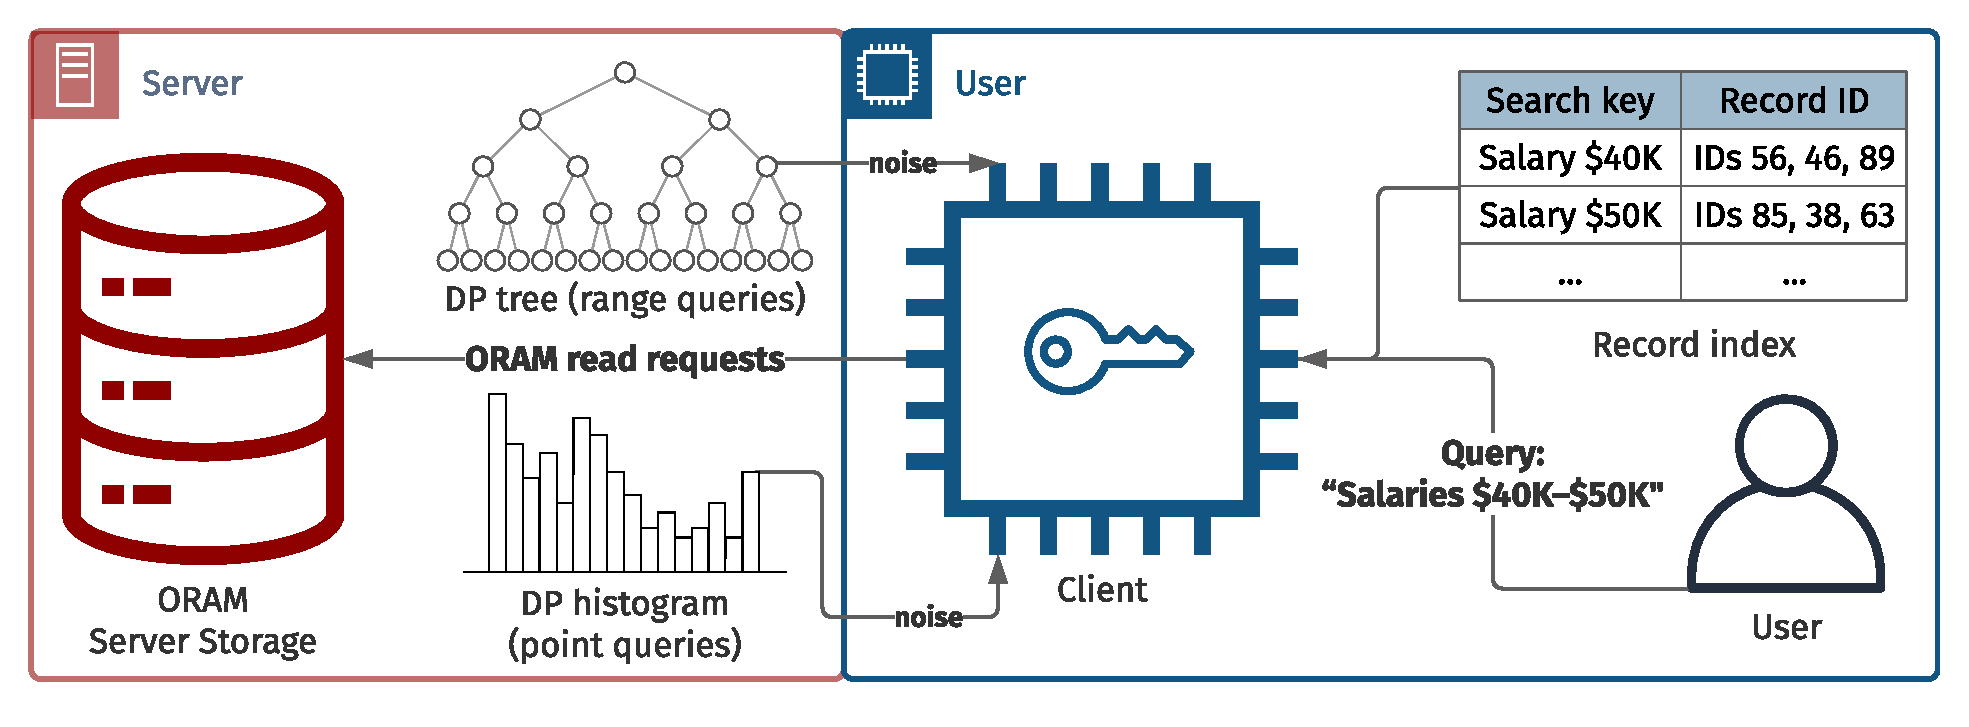
\includegraphics[width=\textwidth]{dp-oram}

	\end{frame}

	\begin{frame}{Parallel \epsolute{}: the choice of separate vs shared \serverDS{}}

		\onslide<1->{
			\begin{itemize}
				\item Split \user{} and \server{} state into \oramsNumber{} ORAMs, run as separate machines
				\item Partition records randomly (by ID) into \oramsNumber{} partitions, generate \oramsNumber{} inverted indexes
				\item Choose a strategy on shared vs split \serverDS{}
			\end{itemize}
		}

		\begin{columns}[T]
			\begin{column}{0.5\textwidth}

				\onslide<2->{
					\begin{block}{No-$\gamma$ method: \serverDS{} per ORAM}

						\begin{itemize}[leftmargin=*]
							\item Composition of disjoint datasets: take max $\epsilon$
							\item Each ORAM replies with $(1 + \gamma) \frac{k_0}{\oramsNumber{}}$ records, where $k_0$ is a required number of records
							\item To bound probability to $\beta$, use $\gamma = \sqrt{ \frac{-3 \oramsNumber \log \beta}{ k_0 } }$
						\end{itemize}

					\end{block}
				}

			\end{column}

			\begin{column}{0.5\textwidth}

				\onslide<3->{
					\begin{block}{$\gamma$-method: shared \serverDS{}}

						\begin{itemize}[leftmargin=*]
							\item Same number of records per ORAM
							\item
								Use $\gamma$ as in no-$\gamma$ method, except
								\begin{itemize}
									\item $k_0 \gets k_0 + \frac{\log \domainSize}{\epsilon}$ for point queries
									\item $k_0 \gets k_0 + \frac{\log^{1.5} \domainSize}{\epsilon}$ for range queries
								\end{itemize}

						\end{itemize}

					\end{block}
				}

			\end{column}

		\end{columns}

	\end{frame}

	\begin{frame}{Parallel \epsolute{} diagram (with improvements)}

		\centering
		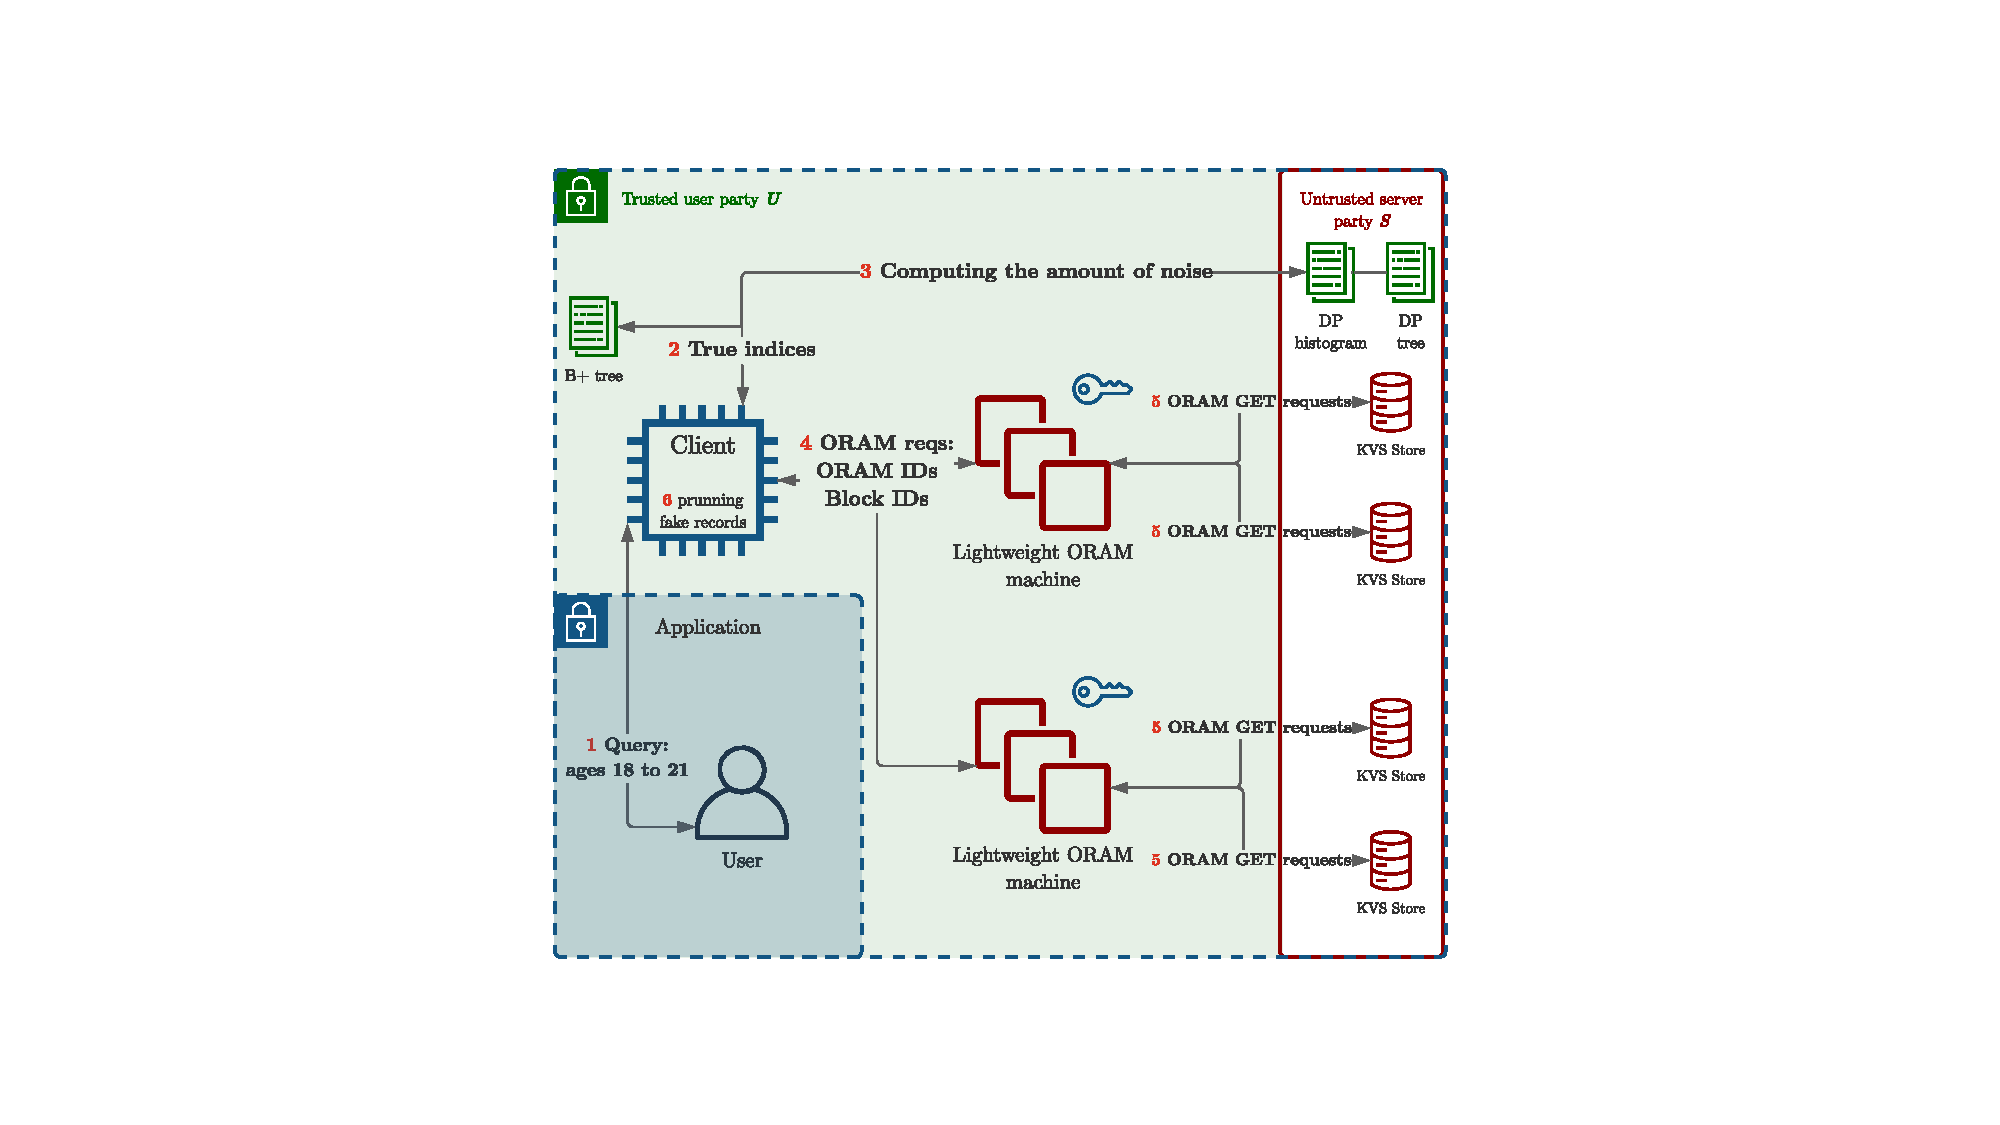
\includegraphics[scale=0.44]{three-layers}

	\end{frame}

	\begin{frame}{Experiments: against other mechanisms}

		\begin{figure}[h]
			\centering
			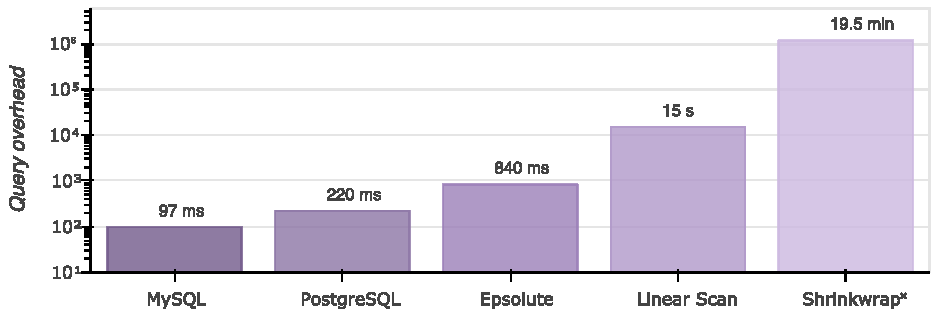
\includegraphics[width=\textwidth]{mechanism}
			\caption{
				\centering
				Different range-query mechanisms (log scale).
				Default setting: $10^6$ \SI{4}{\kibi\byte} uniformly-sampled records with the range $10^4$.
			}%
		\end{figure}

	\end{frame}

	\begin{frame}{Experiments: scalability}

		\begin{figure}[h]
			\centering
			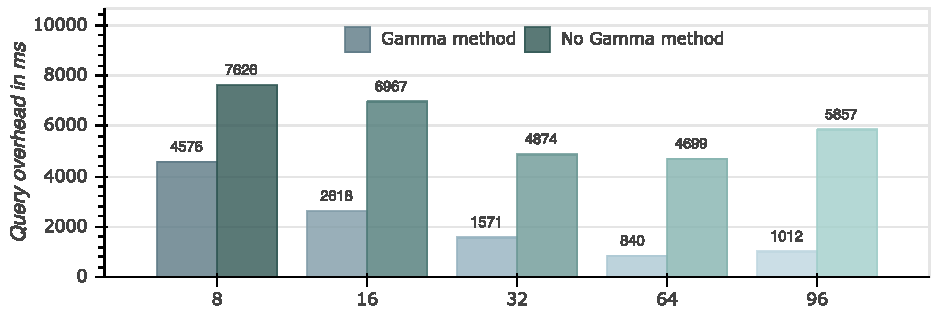
\includegraphics[width=\columnwidth]{scalability}
			\caption{Scalability measurements for \protocolGamma{} and \protocolNoGamma{}}%
		\end{figure}

	\end{frame}


	\maketitle

	\backupbegin%

	\ifthenelse%
		{\equal{\generatenotes}{only}}
		{\nocite{*}}
		{}

	\begin{frame}[allowframebreaks]{References}

		\printbibliography%

		\note{The references}

	\end{frame}

	\backupend%

\end{document}
